\documentclass[
    a4paper,
    12pt,
    oneside
]{report}

% Import packages
\usepackage{graphicx}
\usepackage{subfigure}
\usepackage{amsmath}  % Replaced latexsym with amsmath for symbols and mathematical operations
\usepackage[utf8]{inputenc}
\usepackage[english]{babel}
\usepackage{pdfpages}
\usepackage[
    backend=biber,
    style=ieee
]{biblatex} % IEEE style citations
\usepackage{csquotes}
\usepackage{url}
\usepackage[T1]{fontenc}
\usepackage{float}
\usepackage{palatino}
\usepackage{color}
\usepackage{algorithm}
\usepackage{algorithmic}

\setlength{\doublerulesep}{\arrayrulewidth}
% \setlength{\textwidth}{16cm}
% \setlength{\textheight}{24cm}
% \setlength{\hoffset}{-1.7cm} 
% \setlength{\voffset}{-1cm}
% \setlength{\topmargin}{-0.5cm} 
% \setlength{\footskip}{27pt}
\usepackage[a4paper, margin=2.5cm]{geometry}

\renewcommand{\baselinestretch}{1.3}
\linespread{1}

\usepackage{titlesec}
\titlespacing*{\chapter}{0pt}{-1\baselineskip}{1\baselineskip}
\titlespacing*{\section}{0pt}{\baselineskip}{0pt}

\usepackage{fancyhdr}

\fancypagestyle{noheadrule}{
    \fancyhf{}
    \renewcommand{\headrulewidth}{0pt}
    \renewcommand{\footrulewidth}{0.5pt}
    \fancyfoot[L,LO]{\textit {FINAL PROJECT: Collective Transport using
    Decentralised Swarm Robotics}}
    \fancyfoot[R,RO]{\bfseries\thepage}
}

% Add bibliography file to document
\addbibresource{biblio.bib}

\begin{document}

% Cover
\begin{titlepage}
    \centering
    % \vspace*{1cm}

    {\LARGE \textbf{Final Project I}}\\[1cm]
    {\Huge \textbf{Collective Transport using Decentralised Swarm Robotics}}\\[1cm]

    
\includegraphics[width=0.4\textwidth]{assets/images/ise_logo.png}\\[1cm]
    
    \textbf{Submitted to the}\\[0.1cm]
    Project Committee appointed by the\\
    \textbf{International School of Engineering (ISE)}\\
    Faculty of Engineering, Chulalongkorn University\\[1cm]

    \textbf{Project Adviser}\\[0.1cm]
    Asst.Prof.Paulo Fernando Rocha Garcia, Ph.D.\\[1cm]

    \textbf{Submitted By}\\[0.5cm]
    \begin{tabular}{rl}
        6438067021 & Nattadon Tangsasom \\
        6438075021 & Ting-Yi Lin \\
        6438079621 & Tinapat Limsila \\
        6438118421 & Noppawan Srikhirin \\
        6438187721 & Mehul Sharma \\
    \end{tabular}\\[1cm]
    2/2024: 2147417 Final Project II\\
    Robotics and Artificial Intelligence Engineering (International Programme)\\
    International School of Engineering (ISE) Faculty of Engineering, Chulalongkorn University

\end{titlepage}


\thispagestyle{empty}
\pagenumbering{roman} \setcounter{page}{1}
\setcounter{secnumdepth}{11}
\setcounter{tocdepth}{3}
\renewcommand{\chaptermark}[1]{\markboth{Chapter ~\thechapter~:~#1}{}}
\fancyhf{}
\fancyhead[R,RO]{\bfseries\leftmark}
\fancyfoot[L,LO]{\textit {FINAL PROJECT: Collective Transport using
Decentralised Swarm Robotics}} 
\fancyfoot[R,RO]{\bfseries\thepage}
\fancypagestyle{plain}{
    \fancyhead{}
    \renewcommand{\headrulewidth}{0pt}
} 
\pagestyle{fancy}
\selectlanguage{english}
{\linespread{.8}\tableofcontents}
\newpage
\pagenumbering{arabic}
\titlespacing{\chapter}{0cm}{1cm}{2cm}

% Chapters
\chapter*{Abstract}

\paragraph*{}
This report serves as the proposal for our final project, titled "Collective Transport using Swarm Robotics." It covers various facets of our project, including the project concept, expected outcomes, project timeline, and potential benefits to the industry. Additionally, a comprehensive review of existing literature and a robust theoretical foundation are provided to substantiate our objectives.

\paragraph*{}
Structured into nine chapters, the report begins with an exploration of the research background and our objectives. The literature survey evaluates multiple research papers to identify relevant concepts, enhancing and applying them in innovative ways. Subsequent chapters delve into the development of the project concept, detailing the planning and execution strategy. A theoretical backup section fortifies our project methodology. The anticipated project outcomes are discussed, followed by the potential benefits to the industry. The report concludes by outlining each team member's contributions to the project.

\paragraph*{}
As a proposal for our final project, this report is intended to outline our plans and should not be considered as a finalized product. The comprehensive information provided across the nine chapters aims to furnish sufficient details for an effective project proposal.

\chapter{Introduction}

\paragraph*{}
This progress report aims to highlight the progress of our final project, \textbf{Collective Transport using Swarm Robotics}, with the evaluating criteria being the team individual contributions, as well as our pace in comparison to the ideal schedule. The ideal schedule can be represented by the project Gantt Chart (Figure \ref{fig:gantt_chart}).

\paragraph*{}
According to Figure \ref{fig:gantt_chart}, we are exploring three major sub-tasks during this iteration of the project schedule. These three tasks are: \textbf{Communication in the Swarm} (Task 1.1), \textbf{Object detection using Computer Vision} (Task 1.2), and \textbf{Simple Simultaneous Localization and Mapping} (Task 1.3). These tasks are planned to span for the entire month of September. Two team members, one team member, and two team members are assigned to each task, respectively.

\begin{figure}[H]
    \centering
    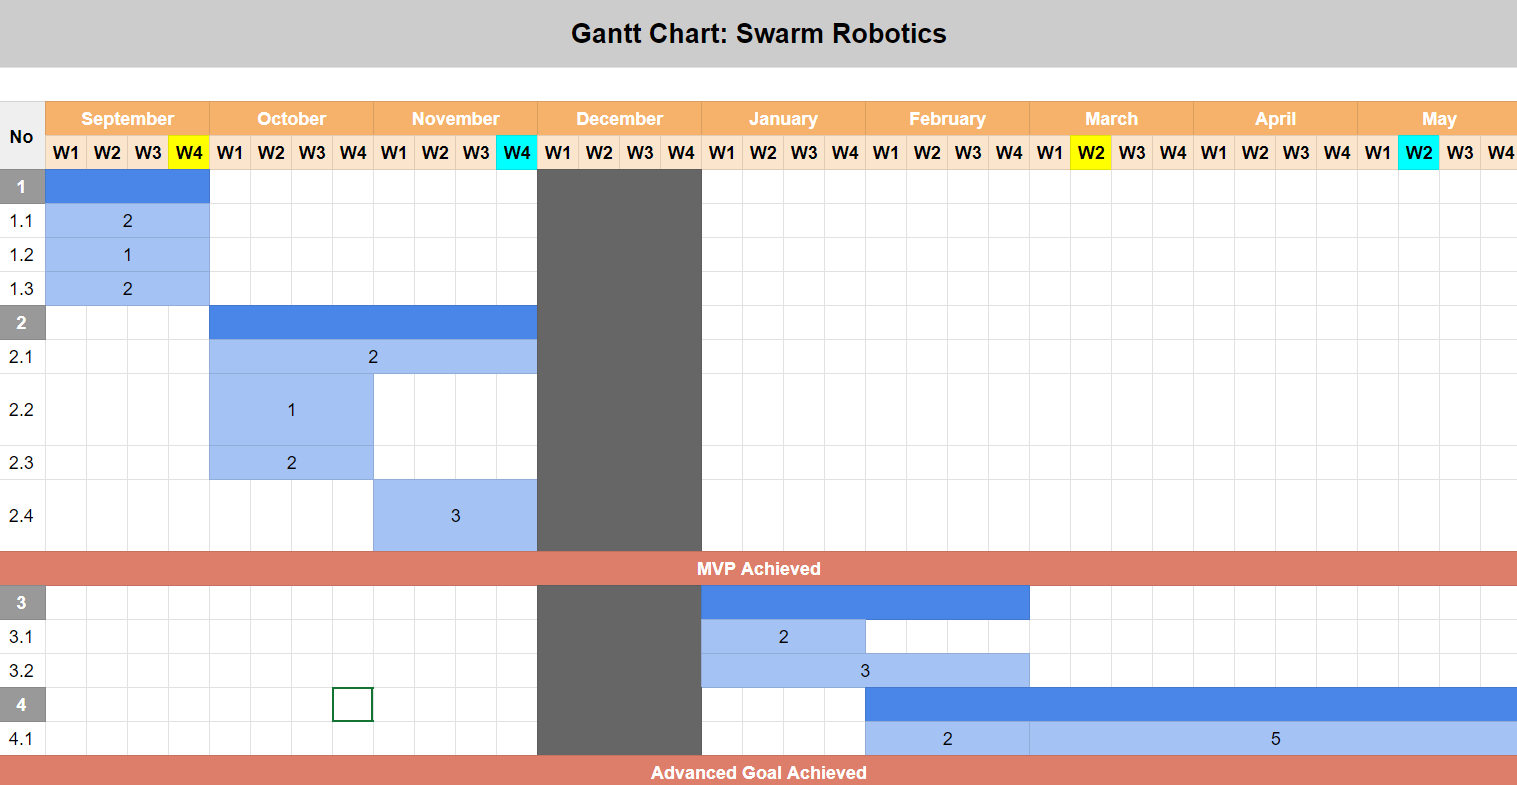
\includegraphics[width=1\linewidth]{progress_report_1/assets/images/introduction/gantt_chart.png}
    \caption{Project Gantt Chart}
    \label{fig:gantt_chart}
\end{figure}

\chapter{Object Detection}

\paragraph*{}
The object detection system initially developed in the previous semester successfully detected a yellow cylinder, generated a bounding box around it, aligned the box’s center with the camera frame, and measured the distance between the robot and the object using the camera’s focal length. However, this implementation relied on the assumption that the cylinder’s dimensions were known, and LiDAR had not yet been integrated. Additionally, the scope of object detection was refined from hexagonal prisms and cubes to cylinders to eliminate the need for pose estimation and edge detection, which would otherwise introduce additional computational complexity for dynamic object grasping.

\paragraph*{}
In transitioning to real-world implementation, several modifications were made to the object detection workflow. The system now identifies three distinct objects: a yellow, a blue, and a red cylinder, each differing in size. At this stage, only a single object is placed in the arena at a time, with detection based primarily on colour. Once detected, the system generates a bounding box around the object, and its distance and size are measured using an S3 RPLiDAR. To enhance accuracy, multi-sensor fusion between the camera and LiDAR is employed. By leveraging the camera’s horizontal field of view (FOV), the system maps the bounding box’s pixel range to the corresponding angle and retrieves the appropriate LiDAR data based on the robot’s odometry.

\paragraph*{}
The current implementation has successfully demonstrated the ability to detect objects based on color while filtering out reflections from the floor. Initial testing was conducted under controlled lighting conditions, including illumination from the left, right, front, and back. The presence of vibrations caused by the camera mount during movement did not significantly affect detection performance. However, at this stage, accuracy assessments are still based on visual inspection, and further validation will be conducted once the model undergoes proper calibration with the sensors. Overall, progress remains on schedule and aligns with the expected timeline, with each milestone being achieved as planned.

\paragraph*{}
In measuring distance and size, image distortion remains a key factor influencing accuracy, as the system must correctly map the detected object’s bounding box angle to real-world coordinates. Since the object’s height does not contribute to measurement calculations, vertical calibration data from the camera has been omitted. Additionally, the top 30 degrees of the camera frame is cropped to remove potential noise and prevent false detections of unintended objects or individuals outside the arena.

\paragraph*{}
One of the primary challenges encountered in this phase is object occlusion, where multiple objects appearing in the frame can lead to overlapping bounding boxes. In such cases, the robot is required to reposition itself to separate the detected objects and ensure accurate size measurements without interference. Another challenge is ensuring reliable color detection under varying lighting conditions, as different light sources and angles can affect how the camera perceives object colors. Additionally, image distortion presents difficulties in mapping the bounding box to the correct position in relation to the LiDAR data. These obstacles are being addressed through careful calibration, adjustments in object positioning, and improvements to the detection algorithm to enhance its robustness against occlusion and lighting variations.

\paragraph*{}
To meet the minimum viable product (MVP) requirements, the initial implementation is limited to detecting a single object within the arena. The system must be capable of generating a bounding box, measuring both distance and angle, and determining the object's size using LiDAR. Once these fundamental objectives are achieved, the next phase of testing will involve detecting multiple objects within a single frame while handling occlusion through coordinated robot movement.

\paragraph*{}
Further testing will focus on optimizing the model and evaluating its accuracy under different conditions. The model will first be validated under the MVP scenario, dealing with only one object, before advancing to a multi-object setting with occlusion management. To assess distance measurement accuracy, objects will be placed at 0.5, 1, and 3 meters from the robot, allowing evaluation of the alignment between LiDAR and camera data. Additionally, eight different lighting conditions will be introduced by positioning the light source at varying angles to examine the robustness of the color detection model under diverse illumination environments.

\documentclass{report}
\usepackage{booktabs}
\usepackage{geometry}
\usepackage{caption}
\usepackage{float} % for [H] placement
\geometry{margin=1in}

\begin{document}

\appendix
\chapter{Object Detection Model Testing Result}

\begin{table}[t]
    \centering
    \caption{Predicted diameter under different lighting conditions of 20 cm diameter cylinder, placed at actual relative angle of 0 degree.}
    \label{tab:20cm}
    \begin{tabular}{cccc}
    \toprule
    \textbf{Lighting Condition} & \textbf{Distance (m)} & \textbf{Angle (°)} & \textbf{Predicted Width (m)} \\
    \midrule
    1 & 0.5 & 0.21 & 0.20 \\
    2 & 0.5 & 0.21 & 0.20 \\
    3 & 0.5 & 0.21 & 0.20 \\
    4 & 0.5 & 0.21 & 0.20 \\
    5 & 0.5 & 0.28 & 0.20 \\
    6 & 0.5 & 0.28 & 0.20 \\
    7 & 0.5 & 0.13 & 0.20 \\
    8 & 0.5 & 0.21 & 0.20 \\
    9 & 0.5 & 0.21 & 0.21 \\
    \cmidrule(lr){1-4}
    1 & 1.00 & 0.37 & 0.20 \\
    2 & 1.01 & 0.43 & 0.20 \\
    3 & 1.00 & 0.43 & 0.20 \\
    4 & 1.00 & 0.37 & 0.20 \\
    5 & 1.00 & 0.43 & 0.20 \\
    6 & 1.00 & 0.31 & 0.20 \\
    7 & 1.00 & 0.29 & 0.20 \\
    8 & 1.00 & 0.33 & 0.20 \\
    9 & 1.00 & 0.33 & 0.20 \\
    \cmidrule(lr){1-4}
    1 & 2.00 & 0.18 & 0.20 \\
    2 & 1.99 & 0.18 & 0.20 \\
    3 & 2.00 & 0.18 & 0.20 \\
    4 & 2.00 & 0.18 & 0.20 \\
    5 & 2.00 & 0.18 & 0.20 \\
    6 & 1.99 & 0.18 & 0.20 \\
    7 & 2.00 & 0.18 & 0.20 \\
    8 & 2.00 & 0.18 & 0.20 \\
    9 & 2.00 & 0.18 & 0.20 \\
    \cmidrule(lr){1-4}
    1 & 3.00 & 0.35 & 0.20 \\
    2 & 3.00 & 0.29 & 0.20 \\
    3 & 3.00 & 0.29 & 0.20 \\
    4 & 2.99 & 0.29 & 0.20 \\
    5 & 3.00 & 0.29 & 0.20 \\
    6 & 3.00 & 0.29 & 0.20 \\
    7 & 3.01 & 0.35 & 0.19 \\
    8 & 3.00 & 0.29 & 0.20 \\
    9 & 3.00 & 0.29 & 0.20 \\
    \bottomrule
    \end{tabular}
\end{table}

\begin{table}[htbp]
\centering
\caption{Predicted diameter under different lighting conditions of 16 cm diameter cylinder, placed at actual relative angle of 0 degree.}
\label{tab:16cm}
\begin{tabular}{cccc}
\toprule
\textbf{Lighting Condition} & \textbf{Distance (m)} & \textbf{Angle (°)} & \textbf{Predicted Width (m)} \\
\midrule
1 & 0.5 & 358.11 & 0.16 \\
2 & 0.5 & 358.11 & 0.16 \\
3 & 0.5 & 358.11 & 0.16 \\
4 & 0.5 & 358.05 & 0.16 \\
5 & 0.5 & 358.11 & 0.16 \\
6 & 0.5 & 358.11 & 0.16 \\
7 & 0.5 & 358.11 & 0.16 \\
8 & 0.5 & 358.11 & 0.16 \\
9 & 0.5 & 358.11 & 0.16 \\
\cmidrule(lr){1-4}
1 & 1.00 & 0.18 & 0.16 \\
2 & 1.00 & 0.18 & 0.16 \\
3 & 1.00 & 0.18 & 0.16 \\
4 & 1.00 & 0.18 & 0.16 \\
5 & 1.00 & 0.12 & 0.16 \\
6 & 1.00 & 0.18 & 0.16 \\
7 & 1.00 & 0.12 & 0.16 \\
8 & 1.00 & 0.18 & 0.16 \\
9 & 1.00 & 0.18 & 0.16 \\
\cmidrule(lr){1-4}
1 & 2.00 & 0.55 & 0.16 \\
2 & 2.00 & 0.61 & 0.16 \\
3 & 2.00 & 0.61 & 0.16 \\
4 & 2.00 & 0.61 & 0.16 \\
5 & 2.00 & 0.55 & 0.16 \\
6 & 2.00 & 0.55 & 0.16 \\
7 & 2.00 & 0.55 & 0.16 \\
8 & 2.00 & 0.55 & 0.16 \\
9 & 2.00 & 0.55 & 0.16 \\
\cmidrule(lr){1-4}
1 & 3.00 & 0.22 & 0.16 \\
2 & 3.01 & 0.28 & 0.16 \\
3 & 3.00 & 0.28 & 0.16 \\
4 & 3.00 & 0.22 & 0.17 \\
5 & 3.00 & 0.28 & 0.16 \\
6 & 3.00 & 0.28 & 0.16 \\
7 & 3.00 & 0.28 & 0.17 \\
8 & 3.00 & 0.28 & 0.16 \\
9 & 3.00 & 0.28 & 0.16 \\
\bottomrule
\end{tabular}
\end{table}

\begin{table}[htbp]
\centering
\caption{Predicted diameter under different lighting conditions of 12 cm diameter cylinder, placed at actual relative angles of 2, 0, 1.5, and 0 degrees.}
\label{tab:12cm}
\begin{tabular}{cccc}
\toprule
\textbf{Lighting Condition} & \textbf{Distance (m)} & \textbf{Angle (°)} & \textbf{Predicted Width (m)} \\
\midrule
1 & 0.5 & 2.01 & 0.13 \\
2 & 0.5 & 2.01 & 0.13 \\
3 & 0.5 & 2.01 & 0.12 \\
4 & 0.5 & 2.00 & 0.14 \\
5 & 0.5 & 2.01 & 0.13 \\
6 & 0.5 & 2.01 & 0.12 \\
7 & 0.5 & 2.02 & 0.13 \\
8 & 0.5 & 2.01 & 0.14 \\
9 & 0.5 & 2.01 & 0.13 \\
\cmidrule(lr){1-4}
1 & 1.00 & 0.21 & 0.12 \\
2 & 1.00 & 0.21 & 0.13 \\
3 & 1.00 & 0.20 & 0.13 \\
4 & 1.00 & 0.21 & 0.12 \\
5 & 1.00 & 0.21 & 0.12 \\
6 & 1.01 & 0.23 & 0.14 \\
7 & 1.00 & 0.21 & 0.12 \\
8 & 1.00 & 0.23 & 0.13 \\
9 & 1.00 & 0.21 & 0.13 \\
\cmidrule(lr){1-4}
1 & 2.00 & 1.65 & 0.12 \\
2 & 2.00 & 1.65 & 0.12 \\
3 & 2.01 & 1.68 & 0.12 \\
4 & 2.00 & 1.65 & 0.13 \\
5 & 2.00 & 1.68 & 0.13 \\
6 & 2.00 & 1.65 & 0.12 \\
7 & 2.00 & 1.65 & 0.12 \\
8 & 1.99 & 1.68 & 0.14 \\
9 & 2.00 & 1.68 & 0.14 \\
\cmidrule(lr){1-4}
1 & 3.00 & 0.05 & 0.12 \\
2 & 3.00 & 0.05 & 0.12 \\
3 & 3.00 & 0.05 & 0.14 \\
4 & 3.01 & 0.05 & 0.12 \\
5 & 3.00 & 0.05 & 0.14 \\
6 & 3.00 & 0.05 & 0.13 \\
7 & 3.00 & 0.05 & 0.12 \\
8 & 3.00 & 0.05 & 0.13 \\
9 & 3.00 & 0.05 & 0.12 \\
\bottomrule
\end{tabular}
\end{table}

\end{document}

\chapter{Conclusion}

\paragraph*{}
Swarm communication has been successfully implemented using a decentralized peer-to-peer architecture facilitated by socket communication. This approach was selected for its low latency and reliability, both of which are essential for real-time data exchange among robots. A three-way handshake mechanism was incorporated to ensure message delivery integrity, along with a consensus algorithm to resolve simultaneous object detection and taskmaster assignment conflicts. With coordinate streaming, dynamic path planning, and task execution now fully integrated, the communication system provides a solid foundation for coordinated swarm behavior, enabling seamless transitions between detection, planning, and movement phases.

\paragraph*{}
Additionally, the object detection system utilizing multi-sensor fusion of the camera and S3 RPLiDAR accurately measures relative distance, relative angle, and estimated width, aided by the variation factor function. This function yields an error margin of 1 centimeter for cylinders with diameters of 16 and 20 centimeters. The model was also tested with objects of different sizes, specifically a cylinder with a diameter of 12 centimeters, resulting in a slightly higher error margin of 2 centimeters. Overall, the object detection component was completed within the expected timeline.

\paragraph*{}
For SLAM we will continue making our own graph SLAM but will work on SLAM Toolbox temporarily. For odometry, we will continue testing and publish results soon.

\paragraph*{}
Meanwhile, the development and testing of our holonomic X-Drive robot have progressed significantly. The robot’s base and structural components were 3D printed using PLA, but to improve durability and stability, key parts such as the baseplate, shaft, wheels, and flange coupler will be upgraded to acrylic and stainless steel. The robot utilizes Dynamixel AX-12W motors for enhanced back-drivability, controlled through a custom ROS 2 package that applies a Jacobian matrix transformation for motion control. Transitioning from the older Maxon BLDC motors has streamlined development, allowing us to focus on software for coordinated multi-robot operation. The successful integration of the teleop keyboard package in ROS 2 Humble has demonstrated holonomic movement, paving the way for further improvements in geometry and performance optimization.

\paragraph*{}
For the next phase of our project, we will complete the tasks that have yet to be completed during the previous iteration and move towards a complete swarm. This includes completing the hardware requirements, considering movement after gripping, as well as testing and evaluation. Additionally, we will proceed with other tasks as scheduled in the Gantt Chart to ensure all project milestones are met.


% Bibliography
\nocite{*}
\printbibliography

\end{document}
